
\chapter{米国の19世紀}



\section{トクヴィル『アメリカのデモクラシー』 (1835)}

アレクシ・ド・トクヴィル (Alexis-Charles-Henri Cl\'{e}rel de Tocqueville, 1805--1859)。


典拠:トクヴィル、『アメリカのデモクラシー』、松本礼二訳、岩波書店、2005, 2008。



\subsection{}



われわれの歴史のページを繰ってみて、この700年の間、大事件といえるもので平等化に役立たなかったものはない。

十字軍と数次にわたる対英戦争は貴族を壊滅させ、その土地を細分化する。自治都市の設立は封建王政の中に民主的自由を導入する。火器の発明は戦場において貴族と庶民の差をなくし、印刷術は人々に平等に知的な糧を提供する。郵便制度は貧者のあばら家にも宮廷にも知識の光を運ぶ。プロテスタンティズムは誰もが平等に天国への道を見出しうるとした。アメリカの発見は一攫千金への新しい途を無数に開き、名もなき冒険家に富と権力をもたらす。

一一世紀から始めて、以後50年ごとにフランスで起こった出来事を調べてみるならば、どの時期の終わりにも社会状態に一つの二重革命が進行しているのを認めざるをえないであろう。社会の階梯を貴族はますます下降し、平民はいっそう上昇する。一方は下がり、他方は上がる。半世紀ごとに両者の距離は縮まり、相接するのはもう間近い。

しかも、これはフランスだけに限られたことではない。どこに目を向けようと、キリスト教世界の全体に同様の革命が続いているのが認められる。

諸国民の生に起こった種々の偶発事は、どこでもデモクラシーの益に帰した。すべての人がこれに尽力した。デモクラシーの勝利のために力を尽くそうと考えていた人も、それに身をささげようとは思ってもみなかった人も。デモクラシーのために闘った人も、自らその敵であると宣言した人さえも。すべての人がひとまとめに一つの途に押しやられ、ある者はその意に反し、他の者は知らぬ間に、神の御手の中にある盲目の道具として力を合わせて働いた。

境遇の平等の漸次的進展はそれゆえ神の御業であり、たしかにその特徴がそこには認められる。すなわち、それは普遍的持続的であり、日ごとに人の力で左右しえぬものとなりつつあり、すべての出来事、すべての人々がその進展に奉仕している。(一・上13-14)

\subsection{}



地域共同体は唯一自然に根ざした社会的結合であって、人間が集まればひとりでに共同体ができるものである。

それゆえ共同社会は慣行、法制を問わず、どんな国民にも存在する。王国を創り国を建てるのは人間であるが、共同体は神の手から直に生ずるように思われる。しかしながら、人間が生まれて以来、地域共同体は存在したとしても、共同体の自由は稀有で壊れやすいものである。一国の人民が大規模な政治集会を組織することはいつでもできる。というのも、人民の中には普通、実務の経験はなくとも、その代わりになるだけの学識をもつ人がいくらかはいるものだからである。地域共同体はしばしば、立法者の働きかけにも耳を貸さぬ粗野な人々で構成されている。地域共同体の独立を確立することの難しさは、国民の知識が開けるにつれて減ずるどころか、むしろ啓蒙とともに増大する。文明の著しく進んだ社会は地域共同体の自由の行使をなかなか許さない。多くの逸脱を見ると我慢できず、実験の最終結果に至る前に成功に絶望してしまう。

地域共同体の自由を確立するのは非常に難しく、またそれはあらゆる自由の中でもっとも権力の侵害の危険にさらされやすい。地域自治の諸制度は、単独では、野心的で強力な政府にとうてい抵抗できまい。うまく自己を守るためには、それは全面的に発達し、国民の思想や習慣と一体化していなければならない。したがって、地域共同体の自由は習俗に基づかぬ限り簡単に破壊される。そして、長い間法の中に生き続けた後でなければ習俗に根づくことはできない。

地域共同体の自由は人間の努力次第でできるというものではない。したがって、それが人の手で創り出されることは滅多になく、いわばひとりでに生まれてくるのである。それは半ば野蛮な社会の中ではほとんど人知れず成長する。法と習俗と環境、なかんずく時間の絶えざる作用がようやくこれを確たるものにする。ヨーロッパ大陸のいかなる国をとってみても、地域共同体の自由を知る国民は一つとしてないといえる。

しかるに、自由な人民の力が住まうのは地域共同体の中なのである。地域自治の制度が自由にとってもつ意味は、学問に対する小学校のそれに当たる。この制度によって自由は人民の手の届くところにおかれる。それによって人民は自由の平穏な行使の味を知り、自由の利用に慣れる。地域自治の制度なしでも国民は自由な政府をもつことはできる。しかし自由の精神はもてない。束の間の情熱、一時の関心、偶然の状況が国民に独立の外形を与えることはある。だが、社会の内部に押し込められた専制は遅かれ早かれ再び表に現れる。(一・上95-97)


\subsection{}



民主主義の諸制度が人の心の中に羨望の念を著しく育てることに目を塞いではならない。その理由は、民主的諸制度が各人に他者と同等になる手段を提供するからというより、それらの手段がこれを利用する人の期待を絶えず裏切るためである。民主主義の諸制度は平等の情念を覚醒し、これに追従するが、決してこれを完全に満足させることはできない。この完全な平等は、民衆がこれを捉えたと思ったその瞬間にいつもその手から逃れ、パスカルが言うように永遠の遁走を繰り返す。認識しうるほどには手近く、味わうには遠すぎるだけに、一層貴重なこの幸福の追求に民衆は熱中する。彼らは成功の望みによって駆り立てられるが、勝利が確かではないので苛立つ。興奮し、疲れ、そして憤る。こうしてなんらかの点で自分より上にある者はすべて自分の欲求の障害と思われ、上に立つのが当然と認めざるをえない人物でも、目の当たりに見れば嫌になる。(一・下55)


\subsection{}


一般に自由な国民はそうでない国民に比べて、危機においてはるかに大きな力を発揮することは疑いない。だがこれは、自由な国民でもその中に貴族的な要素が支配的な場合に特に正しいのではないかという気がする。民主政治は平和な社会を指導し、また必要な場合、急遽、懸命の努力を行なうにはよいが、国民の政治生活の激動を長期にわたって乗り切るにはそれほど適していないように思われる。その理由は単純である。人は熱狂に駆られて危険や窮地に身を投じるとしても、長期間危険と戦うには熟慮がなければならない。本能的な勇気と呼ばれるもののなかにさえ、人の考える以上に計算があるものである。一般に最初の努力は情熱だけでなしうるとしても、持続するには結果を考えねばならぬ。残りを救うために、貴重なものの一部を危険にさらすということもある。

知識と経験に基礎づけられたこの将来への見通しこそ、まさに民主政治にしばしば欠けるものに違いない。人民は理性よりはるかに感情で動く。そして、もしいま現在の苦痛が大きいとすれば、人民は敗北の暁におそらく彼らを待ち受けている、より大きな苦痛を忘れてしまう恐れがある。(一・下97-98)

\subsection{}


政治において人民の多数は何事をもなす権利を有するという原理は、不遜で憎むべきものだと思う。にもかかわらず、私は多数の意志にあらゆる権力の起源を認める。これは自己矛盾であろうか。

特定の国民における多数にとどまらず、すべての人間の多数が定め、少なくとも採用した普遍の法が存在する。それは正義の法である。

すなわち正義は、個々の人民の権利に限界を付すものである。

一国の国民は、人類普遍の社会を代表して、その法たる正義の実現にあたる陪審員のようなものである。社会を代表してその法を適用する陪審員が、社会それ自体より大きな力をもつべきであろうか。

すなわち、不正な法への服従を拒否するとき、私は多数者の命令権を否認するわけではない。ただ人民主権から転じて、人類の主権に訴えるだけである。

人民が己れの利害にしか関わらぬ案件において正義と理性の枠を完全に踏み外すことはありえず、したがって人民を代表する多数者に全権を委ねるのを恐れるべきではないと言って憚らなかった人々がいる。だが、これは奴隷の言葉である。

多数者を一体として見れば、少数者という別の個人と、意見、またたいていの場合、利害において対立している個人にほかならない。ところで、一人の人間が全能の権力を身につければこれを敵に対して濫用するかもしれぬと考えるのであれば、どうして同じことが多数者についても生じることを認めないのか。人間は団体になって性格が変わったのか。力を増すにつれて、反対に対して忍耐強くなったのか。そんなことは私には信じられない。一人の同胞に対して否定する、すべてをなしうる力の保持を、複数の人間だからといって認めようとは決して思わない。(一・下146-148)

\subsection{}


私はアメリカで正直なところこれまで想ってもみなかったような結社に出会い、合衆国の住民が手段を尽くして共通の目標の下に多数の人々の努力を集め、しかも誰もを自発的に目標の達成に向かわせる、その工夫にしばしば賛嘆の声をあげた。

私はその後イギリスを旅行した。アメリカ人はその法制のいくつかと慣習の多くをこの国から受け継いだのであるが、ここではアメリカのように結社を絶えず、また巧みに活用しているようにはとても見えなかった。

イギリス人は非常な大仕事を一人で行うことがあるのに対し、アメリカ人はどんなに小さな事業にも団体をつくる。前者が結社を行動の一つの有力な手段と考えているのは明らかだが、後者は行動するための唯一の手段と見ているかにみえる。

このように地上でもっとも民主的な国はまた共通の欲求の対象を共同で追求する技術に今日もっとも習熟し、この新しい知識をこの上なく数多い目的に適用してきた国である。このことは偶然の結果だろうか、それとも結社と平等の間には必然の関係が事実あるのではなかろうか。

貴族社会の中にはつねに、自分では何をなす力もない無数の人々に囲まれて、きわめて大きな力と富を有する少数の市民が存在する。この人々は誰もがたった一人で大きな事業をなす力をもっている。

貴族社会にあっては、人々が全体として固く結びついているから、行動するために結社をつくる必要がない。

そこでは、富と力を有する市民が、それぞれ、恒久的で脱退できない一つの結社の長のようなもので、この結社の構成員はすべて彼に従属させられ、彼の計画の実現に協力させられている。

ところが、民主的な国民にあっては、市民は誰もが独立し、同時に無力である。一人ではほとんど何をなす力もなく、誰一人として仲間を強制して自分に協力させることはできそうにない。彼らはだから、自由に授け合う術を学ばぬ限り、誰もが無力に陥る。

民主的な国に住む人々が政治的目的のために団体をつくる権利と趣味をもたないとすれば、彼らの独立は大きな危険にさらされるであろう。それでも、富と知識とは長く維持することができるかもしれない。だが日常生活の中で結社をつくる習慣を獲得しないとすれば、文明それ自体が危機に瀕する。私人が単独で大事をなす力を失って、共同でこれを行う能力を身につけないような人民は、やがて野蛮に戻るであろう。(二・上189-191)

\subsection{}


境遇が国民全体の中でますます平等になるにつれて、工業製品の需要がそこに広がり、増大し、そうした製品を財産の少ない人々の手に行き渡らせる低価格の実現は成功の一層大きな要素となる。

そこで、毎日のように、豊かで見識ある人々ほどその富と知識を産業に動員し、大工場を開き、労働の分業を厳密に実行して、至るところに生まれる新たな欲求を満たそうと試みることになる。

したがって、国民全体がデモクラシーに向うにつれて、産業に従事する特別の階級はより貴族的になる。人々は一方でますます類似したものになり、他方では違いがより大きくなり、不平等は社会全体を大きく見れば減少するが、それに比例して小さな社会では増大する。

つまり、根源に遡ってみると、デモクラシーのまさに中心に本来ある一つの動きから貴族制が生じることが分かる。(二・上272)


\subsection{}



一国の人民の習俗が厳しさを和らげるのに与る要因はいくつかあるが、私にはもっとも強力な要因は境遇の平等であるように思われる。境遇の平等と習俗の穏和化はだから私の目には同時進行の出来事というだけでなく、相関する事実と映る。(二・下13)

\subsection{}



一国の人民の中で地位がほぼ平等であるとき、誰もがほぼ同じような考え方、感じ方をするから、誰にとっても他のすべての人の感覚を瞬時に判断することができる。自分自身を一目振り返れば、それでよいからだ。だからどんな不幸も簡単に理解でき、隠れた本能がその大きさを教える。未知の他人や敵だからといって変わりはない。想像力を働かせれば、そういう人の身にもすぐなれる。想像力は哀れみの情に何ほどか個人的な感情を紛れ込ませ、仲間の身体が痛めつけられれば、わが身に苦痛を覚える。

民主的な世紀には、人が人のために身を犠牲にすることは滅多にないが、人類全員に広く思いやりを示す。無益な苦痛を他人に与えることはなくなり、自分をたいして害することなく他人の痛みを軽減できるときには、喜んでそうする。人々は無私ではないが、心優しい。(二・下19-20)

\subsection{}




デモクラシーの人々は生来革命を望まないだけでなく、これを恐れる。

既得の財産を多少とも脅かすことのない革命はない。民主社会に住む人々の大半は財産所有者である。彼らは財産所有者であるだけでなく、人々が財産に最大の価値を付与する状況に生きている。

社会を構成する諸階級を一つ一つ注意深く考察するならば、財産所有から生まれる情念が中産階級におけるほど激しく執拗である階級はないと容易に分かる。

しばしば貧乏人は自分の所有物に執着しないが、それは彼らにとって物がない苦しさの方が僅かばかりの持ち物から得る喜びよりもはるかに大きいからである。金持ちには富の情熱の他に満たすべき多くの情熱があり、さらに、大きな財産を長期間苦心して運用する間に、彼らは時として大財産の効用に無感覚になってしまうことがある。

だが、富裕からも貧困からも等距離の程よいゆとりの中に暮らす人々は自分の財産に計り知れない価値をおく。彼らはまだ貧しさのすぐ隣にいるので、貧困の厳しさを間近に見ており、これを怖れる。貧困と彼らを隔てるものはささやかな家産だけであり、彼らはやがて恐怖と希望の念をそれに込める。家産の維持を常時心がけることで一層それへの関心を大きくし、これを大きくしようと日々努めることによって執着は刻々増していく。ほんの僅かでも家産を譲り渡すという考えは耐え難く、全部失うことは最悪の不幸とみなす。そして、このような熱に浮かれて不安を抱えた小所有者の数を境遇の平等は不断に増大させる。

したがって、民主社会では、市民の多数にとって革命が起こって何の得があるかは明らかでなく、革命があれば何を失うことになるかは、刻々、さまざまな形で感得できる。(二・下158-159)



     \begin{figure}[htbp]
       \centering
         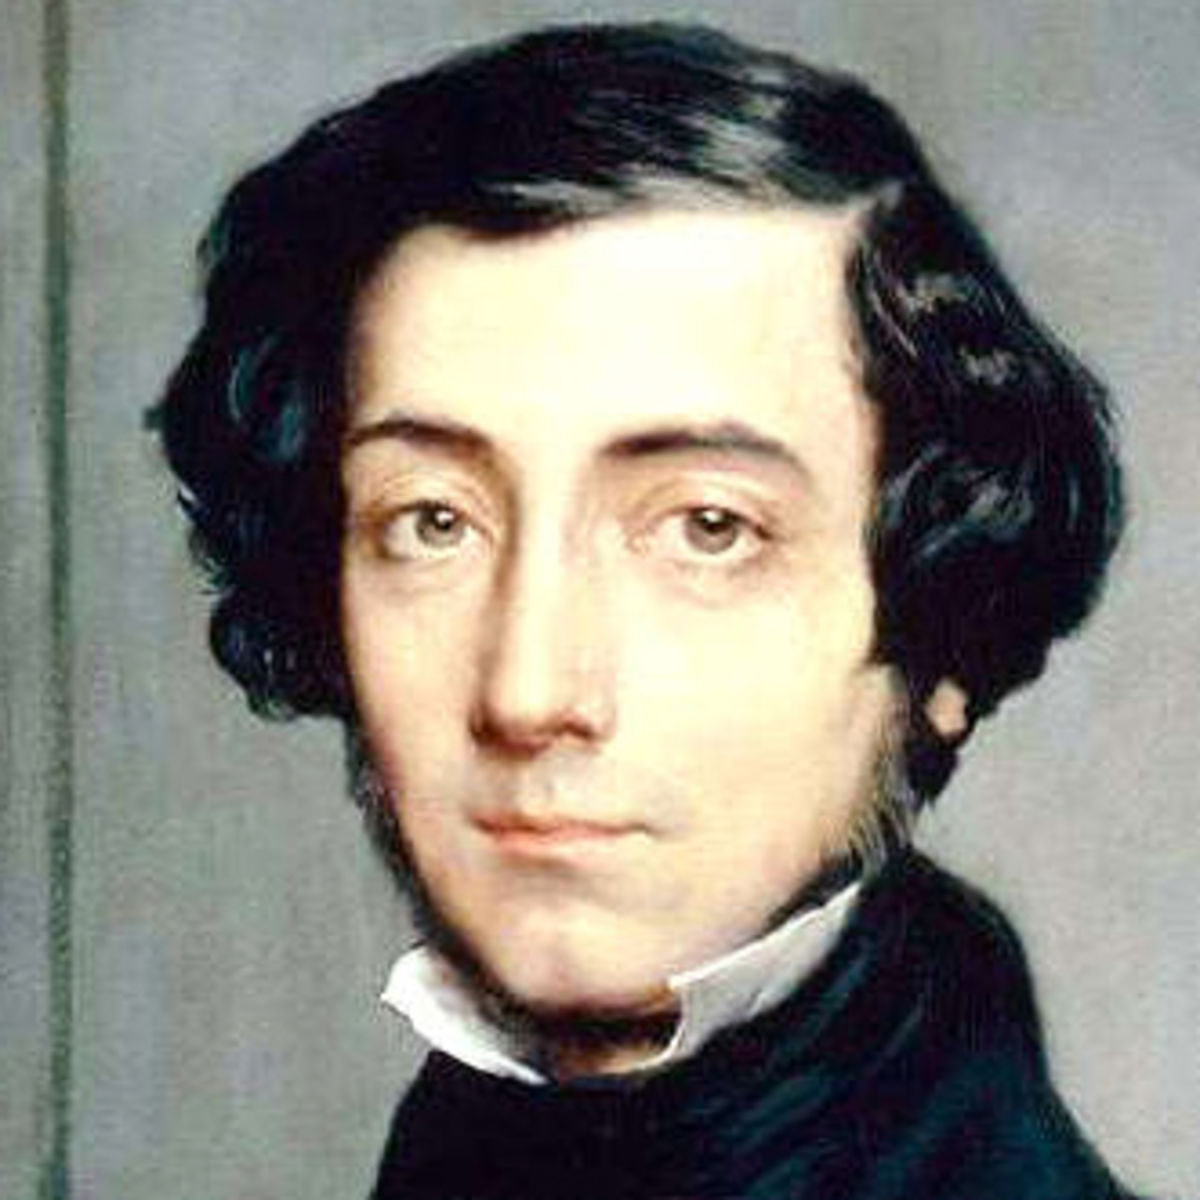
\includegraphics[width=50mm]{images/tocqueville.jpg}
       \caption{トクヴィル}
     \end{figure}



\pagebreak{}


\section{セネカ・フォールズでの「女性の所信宣言」  (1848)}

\label{sentiment}

1848年、米国ニューヨーク州のセネカ・フォールズで開かれた最初の女性の権利の獲得のための胥議。300名程度が参加し、米国の女性解放運動の出発点とされる。エリザベス・スタントンが起草した「女性の所信宣言」などが採択された。

\subsection{}




人類の歴史の過程におき、それらのうちのある一部の人々が、従来占めていた地位と異なりはするが自然法と自然の神の法が彼らに授けた地位を、世界の人々のなかで占めなければならなくなった時に、人類が行ってきた意見表明に対して当然の敬意を払おうとするならば、なぜ自分たちがそのような道程を取らざるを得なくなったかという理由をその人々は宣言すべきである。

よって、わたしたちは、以下の真実を自明の理として宣言する。すべての男性とすべての女性は平等に造られていることを、彼らはともに造物主によって一定の不可譲の諸権利を賦与されていることを、これらの諸権利のなかには、生命、自由、幸福の追求の権利が含まれていることを、これらの諸権利を保障するために政府は創設され、その正当な権力は被治者の同意に由来することを。これらの目的に害をなす政府があるならば、その政府に対する忠誠を拒否し新しい政府の創設を主張することは、その政府に忍従を余儀なくされている人々の権利である。新しい政府は、彼らの安全と幸福にもっとも効果があると思われる諸原則に基礎を置き、そのような形体へと政府の権限を組織するものでなければならない。たしかに、長く存続した政府が軽微で一時的な事由で変更を受けるべきではないことは、分別の命じるところではあるのだが、その結果のすべての経験が示すところは、人間には、自分たちが慣れ親しんできた形体を廃止してあるべき状態に戻るよりは、害悪に耐えうる間はこれに耐える傾向がある、ということである。しかしながら、常に同じ目的を果たすための長期にわたる一連の権力の濫用と簒奪が、人々に絶対的な専制を強いようとする意図を明らかにする場合には、その政府を捨て去り自らの将来の安全のために新しい防護の組織を備えることこそが、人間の義務である。そして、現在の政府のもとで女性たちが耐えてきた忍従こそ、まさにそのような忍従だったのであり、また、本来その資格がある平等な地位を女性たちが今この時要求せざるを得ないのは、まさにそのようなやむにやまれぬ必要性からなのである。

人類の歴史は、女性に対する男性の絶対的な専制の確立を直接の目的とした、男性による女性に対しての権利侵害と剥奪の繰り返しの歴史である。これを証明するために、公平なる世界に向けて、以下の事実を明らかにしよう。

男性は、不可譲の権利である選挙権の行使を、決して女性に認めてこなかった。

男性は、女性がその制定過程に何の発言権も持っていない法に、女性を従わしめようとしてきた。

男性は、もっとも無知で身分が低い男性であろうとも、自国民であるか外国人であるかを問わず与えられている諸権利を、女性には制限してきた。

男性は、選挙権という市民として第一の権利を女性から奪い、それによって立法府で女性が代表されないままにしておくことによって、女性をあらゆる面から抑圧してきた。

男性は、女性が結婚した場合には、法律的に民事上の無能力者としてきた。

男性は、女性が自ら働いて得た賃金をも含むあらゆる財産上の権利を、女性から奪ってきた。

男性は、多くの犯罪を、夫の面前で行われたならば妻がそれらの罪を犯しても不可罰にすることで、女性を道徳的に責任を取れない存在にしてきた。法が妻の自由を奪い貞操を管理する権限を夫に与えたせいで、婚姻契約において妻は夫への恭順を約束することを余儀なくされ、夫は事実上、妻の主人となっているのである。

男性は、離婚法を制定するに際し、何が離婚の正当な事由となるかについて、また別離の場合に誰に子供の監護権が与えるかについて、女性の幸福には一顧だにしなかった。離婚法は、すべての場合において、男性の優位という誤った前提に立っており、男性の手にすべての権力を委ねているのである。

男性は、既婚女性としてのすべての権利を女性から奪っただけでなく、女性が独身で不動産を所有する場合には、税を課して政府を支えさせるが、政府がこの女性の存在を認めるのは、彼女の財産が政府にとって利益を生じるときのみである。

男性は、利益のある仕事のほとんどすべてを独占してきたのであり、女性が就くのを許された仕事からは、女性はほんのわずかの報酬しか得られない。男性は、女性に対し、男性によって最も名誉あると思われる冨と特典へのあらゆる道を閉ざしている。名を知られた神学、医学、法学の教師は、女性にはひとりもいない。

男性は、女性が十分な教育を受ける機会をなくしてきた。あらゆる大学教育は、女性に門を閉ざしている。

男性は、使徒伝の権威を理由に、いくつかの例外はあるが教会の職務への公的な参加から女性を排除したり聖職から女性を排除することによって、国家において従属的地位しか与えなかったのと同じように教会においても従属的な地位しか、女性に与えてこなかった。

男性は、男女で異なる道徳律を世の中に示すことにより、人々に誤った道徳観を創り出した。この道徳律へに違反すれば、女性は社会から締め出されるが、男性の場合は、許容されるだけでなくほとんど問題にされない。

男性は、女性の行動範囲を定め得るのはその女性の良心と彼女の信じる神のみであるにもかかわらず、これを自分たち男性の権利であると主張して、エホバその人の特権を奪い取ってきた。

男性は、為しうるかぎりのあらゆる方法でもって、自分たちの力についての女性の自信を砕き、女性の自尊心を弱め、女性が従属的で屈辱的な人生に甘んじるように努めてきた。
  

さて、この国の半分の人々が選挙権を完全に奪われ、社会的にも宗教的にも劣位におとしめられていることを考慮し、また上記のような不正な諸法を考慮し、さらに、女性たちが、虐げられ抑圧され自分たちの最も神聖な諸権利を不正に奪われていると感じているがゆえに、わたしたちは、合衆国市民として女性に属するすべての権利と特権が、直ちに女性たちに認められるべきであると主張する。
  
わたしたちの目の前にある偉大な事業を始めるにあたり、かなりの誤解や間違った理解、嘲笑を受けるだろうことを予想している。しかし、わたしたちは、自分たちの目的を達成するために、できる範囲のすべての手段を利用するつもりである。わたしたちは、職員を雇い、パンフレットを配布し、州と連邦の立法府に請願し、聖職者と出版界に私たちへの協力を要請するよう努める。わたしたちは、この会議に続き、この国の各地で次々と同じような会議が続かんことを希求する。



\subsubsection*{決議}





(以上に鑑み、)自然の偉大なる教えが、「人間はその人自身の真の実質的幸福を求める」ということであることは、広く知られている。ブラックストーンは著書の「法律釈義」のなかで、この自然法は、人類と同じくらい古く、神ご自身が命じたものであって、当然あらゆる義務に優越する、と述べている。自然法は、世界中で、あらゆる国々で、あらゆる時代において、人々を拘束する。人間の法の中でこの法に背く法は、何の効力も持たず、一方、効力のある法は、その力のすべて、その効力のすべて、その権威のすべてが、直接的にも間接的にも、本来の法であるこの自然法に由来するのである。ゆえに、わたしたちは、以下のことがらを決議する。
  
自然の教えこそが「あらゆる義務に優越する」がゆえに、いかなる形であれ女性の真なる実質的幸福に相反するような法は、自然の偉大なる教えと矛盾するものであることを、決議する。

自分たちの良心にかなった社会的地位を女性が占めるのを阻んだり、男性の地位よりも劣った地位に女性を位置づけたりするあらゆる法は、偉大なる自然の教えに反しており、ゆえに何の力も権威も持たないことを、決議する。

女性は男性と対等であり、造物主によってそのように作られており、人類の至高の徳に従うならば女性はそのようなものとして認められるべきことを、決議する。

この国の女性たちが、彼女らがそのもとに生きる法について知識を得るべきこと、また彼女らが、現在の自分の地位で満足だと宣言することで自分たちの卑しい地位を明らかにしてしまったり、自分が望んでいる権利はすべて手にしていると主張して無知をさらけだしたりすることがないようにと、決議する。

男性が自分たちの知的優越性を主張する一方で女性に道徳的優越性を与えていることに鑑みれば、あらゆる宗教的な会合において機会がある場合には、女性が演説し説教するように推奨することは、まったくもって男性の義務であることを、決議する。

社会において女性に求められるのと同じだけの貞淑さ、繊細さ、洗練が、男性にも求められなければならず、これを破った場合には、男性にも女性にも同じだけの厳しさで対応がなされねばならないことを、決議する。

女性が聴衆に向けて話しかけたときにしばしば投げかけられる不躾で不作法な非難の声は、女性を力づけようという気持ちでステージ、コンサート、サーカスでの女性の演技や発表を見に来ている人たちからは、生じるべくもないものであることを、決議する。

聖書の歪曲した適用によって生じたものであり、市民の心を腐敗させてしまう厳しい制約に対して、女性はあまりにも長い間不満を覚えずにいたのであるが、今や、偉大な造物主が彼女に課したより大きな領域へと動かねばならないときが来たことを、決議する。

選挙権という女性の神聖な権利を確実に手にすることが、この国の女性たちの義務であることを、決議する。

人権の平等は、人間が持つ能力と責任が[性にかかわらず]同じものであるという事実から、必然的に帰結するものであることを、決議する。

ゆえに、以下を決議する。造物主によって自分たちの行為に関して[男性と]同一の能力と同一の責任を与えられているのであるから、あらゆる正当な手段によってあらゆる正当な主義主張を訴えていくことが、男性同様女性の権利であり義務であることは明らかである。とりわけ、道徳と宗教という重要な課題に関しては、私的生活においても公の場においても、利用に問題のないあらゆる手段を利用し、開催に問題のないあらゆる集会で、文章を書いたり公演したりすることで、男性の同胞とともにこれらの課題にかんして啓蒙を行うことに参加するのが、女性の権利であることは自明である。そして、これらのことは、神に教えられた人間の本性の諸原則から生じた自明の真理であり、これらに反するどのような習慣や権威も、近代のものであれ恐ろしい制裁を伴う古代のものであれ、自明の誤りとみなされ、人類の存在とあい争うものなのである。

[最後の会合で、ルクレシア・モットは、次の決議を提案し取り上げた。]

われわれの主張が迅速に達成されるためには、聖職の独占の打倒を求めての、また、さまざまな交易、専門職、商業に対し、男性と平等な参加を女性に保障することを求めての、両性によるところの熱心でたゆまぬ努力が必要であることを、決議する。
\begin{flushright}
  (澤敬子訳)
\end{flushright}


  \begin{figure}[htbp]
    \centering
      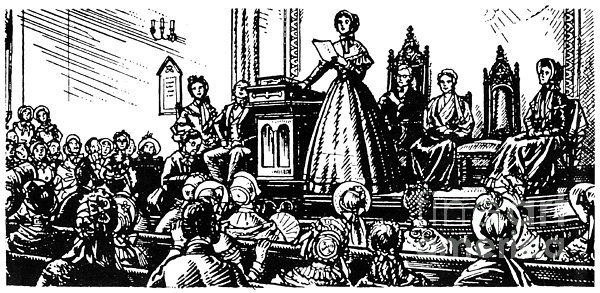
\includegraphics[width=75mm]{images/seneca-falls.jpg}
    \caption{セネカフォールズ会議}
  \end{figure}





% \section{ソジャーナ・トルースの演説}
% \label{truth}
% 「白人男性はやがて権利について話し合っている南部の黒人と北部の女性の間で板挟みになるだろう。しかしここで一体何について話しあっているのかい。あの向うにいる男性は、女が馬車に乗るのに手を貸したり、抱き上げて溝を渡したり、いたるところで一番いい場所を譲る必要があると言っている。今までだれも私を馬車に助け上げてくれたり、田圃から引っ張り上げてくれたり、最上の場所をくれたりはしなかった。私は女じゃないのかい。見てご覧、私の腕を・・・土を耕し、苗を植え、収穫を納屋へ運んで働いてきた。男だって私には勝てない。それでも私は女ではないのかい。私は男と同じくらい働き、男と同じくらい食べることができる。そして同様に苦痛に耐えることができる。だからって、私は女ではないのかい。私は13人の子どもを生み、みんな奴隷に売られていった。泣き叫んでもイエス様以外だれも私の叫びを聞いてくれなかった。それでも私は女ではないのかい。

% そこの黒い服を来た小さな男の牧師は男と同じ権利を持つことはできない、なぜならキリストは女ではなかったから、と云う。キリストはどこからきたんだい。・・・神様から、そして女から生まれたのだ。男は神とはなんの関係もなかった。(後略)」

% \begin{flushright}
%   (奥田暁子訳)
% \end{flushright}




\pagebreak{}

\section{ソロー「市民の反抗」(1849)}


ヘンリー・デイヴィッド・ソロー (Henry David Thoreau, 1817--1863)。


出典:ソロー、「市民の反抗」、『市民の反抗』、飯田実訳、岩波文庫、1997。

\subsection{}

不正なる法律が存在する。われわれは甘んじてそれに従えばいいのか、あるいは、それを修正しようとつとめながら、われわれの試みが成功するまではそれに従うほうがよいのか、それともただちに法を犯すほうがよいのか? 現在のような政府のもとにあっては、たいていの人間が、多数者を説得して法律を快晴させるまで待つべきだ、と考えている。彼らによると、へたに抵抗すれば、その矯正手段のほうが悪法以上にわるい結果を招くというのだ。しかし、矯正手段のほうが悪法よりもわるいというのが\kenten{事実}だとすれば、それこそ政府自体の欠陥である。\kenten{政府}が、それをわるくしているのである。……(25)

\subsection{}

私が確信するところでは、もし千人、といわず百人が、あるいは、私が名前を挙げることのできる十人{\——}たった十人の\kenten{誠実な}人間{\——}が、たった\kenten{ひとり}の「誠実な」人間が、このマサチューセッツ州での\kenten{奴隷の所有をやめ}、政府との共犯関係からきっぱりと身をひき、そのために郡刑務所に監禁されるならば、そのことが取りも直さずアメリカにおける奴隷制度の廃止となるであろう。ことのはじまりがどれほど小さくみえようと、少しも問題ではないのであて、ひとたび立派になされたことは、永久にんされれたのである。ところがわれわれは、この問題について議論するほうを好み、そうすることがわれわれの使命だ、などと言っている。改革に奉仕する新聞は何十とあるのに、改革に奉仕する人間はひとりもいない。(29-30)

\subsection{}

われわれは、自己の投票権のすべてを行使すべきである。単なる一片の投票用紙ではなく、自己の影響力のすべてを投じるべきである。多数派に迎合しているかぎり、少数派は無力だ。その場合、彼らは少数派でさえない。しかし少数派が全力をあげて妨害するとき、彼らにかなう者はいない。もし、すべての正しい人間を獄中に閉じこめておくか、それとも戦争および奴隷制度を放棄するかの二者択一を迫られたならば、州は選択をためらったりはしないだろう。仮に千人が今年の税金を支払わないとしても、それは税金を支払うことによって州に暴力をふるわせ、無実の血を流させることほどには、暴力的で血なまぐさい手段であるとはいえないだろう。……


  \begin{figure}[htbp]
    \centering
      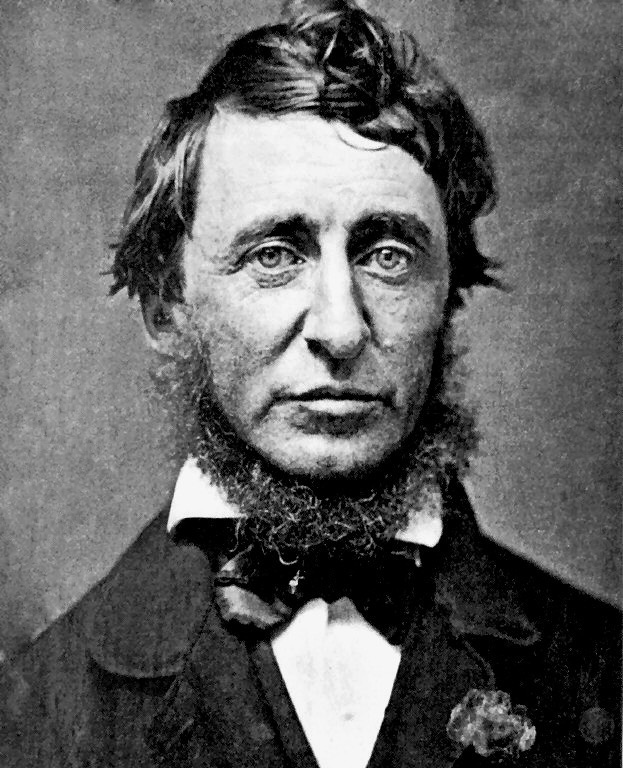
\includegraphics[width=50mm]{images/thoreau.jpg}
    \caption{ソロー}
  \end{figure}



\section{推薦図書}




\begin{itemize}
\item 富永茂樹 (2010)『トクヴィル:現代へのまなざし』岩波書店。ハイブラウな新書。トクヴィルという人物の複雑さがよく伝わる。(渡)

\end{itemize}

%%% Local Variables:
%%% mode: japanese-latex
%%% TeX-master: "main_gendai"
%%% coding: utf-8
%%% End:
